\documentclass{article}
\usepackage[utf8]{inputenc}
\usepackage[margin=1in]{geometry}

\title{518 - Assignment 2}
\author{Victor Zhang}
\date{----}

\usepackage[utf8]{inputenc}
\usepackage{amsmath}
\usepackage{amsfonts}
\usepackage{natbib}
\usepackage{graphicx}
% \usepackage{changepage}
\usepackage{amssymb}
\usepackage{xfrac}
% \usepackage{bm}
% \usepackage{empheq}
\usepackage{dirtytalk}
\usepackage{tikz}

\newcommand{\contra}{\raisebox{\depth}{\#}}

\newenvironment{myindentpar}[1]
  {\begin{list}{}
          {\setlength{\leftmargin}{#1}}
          \item[]
  }
  {\end{list}}

\pagestyle{empty}

\tikzset{every picture/.style={line width=0.75pt}} %set default line width to 0.75pt

\begin{document}

\maketitle
% \begin{center}
% {\huge Econ 482 \hspace{0.5cm} HW 3}\
% {\Large \textbf{Victor Zhang}}\
% {\Large February 18, 2020}
% \end{center}

\section{Introduction}
The purpose of this assignment is to augment our existing thread implementation
with a memory management system. The design specifies a \say{main memory} size
of 8MB and \say{disk} size of 16MB. Because of nice properties we can exploit
with these sizes, we build our memory management system under the strict
assumption of 8MB main memory and 16MB disk. That is, it is not easily scalable
to any larger size of memory or disk. The drawback is obvious, but the advantage
is this allows us to be extremely compact in our metadata. In addition, we work
under the assumption of 4k pages. Since this is essentially the the standard
everywhere (unless using hugepages), we feel this is a reasonable assumption to
make.

\section{Phase 1}
For this phase, the main task is to efficiently allocate memory within a page.
We use a segmented paging strategy implemented using a linkedlist. We allocate
in blocks of size 64 bytes (a typical cache line), meaning there are
$4096/64 = 64$ blocks in each page. For each segment, we keep one byte of
metadata. Figure \ref{fig:segment_metadata} shows this. The top bit represents
the status of the segment, \verb|1| for occupied, \verb|0| for free. The rest of
the bits represent the length of this segment. But a segment can have length 64,
which requires 8 bits to represent! We solve this problem by introducing
\textit{normalized lengths}. Since each segment will have length at least 1, it
makes no sense to start counting from 1. A normalized length of 0 will
correspond with an actual length of 1 block. In general, a normalized length of
$k$ corresponds with an actual length of $k+1$ blocks. This  allows us to
represent the length of a completely free page (64 blocks) in 7 bits instead of
8. So remarkably, we can fit all of our necessary metadata within one byte.

\begin{figure}
\centering
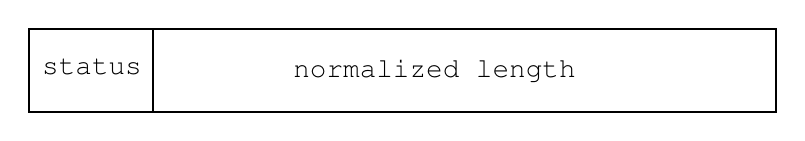
\begin{tikzpicture}[x=0.75pt,y=0.75pt,yscale=-1,xscale=1]
\draw   (190,50) -- (550,50) -- (550,90) -- (190,90) -- cycle ;
\draw    (250,50) -- (250,90) ;
\draw (195,63) node [anchor=north west][inner sep=0.75pt]   [align=left] {{\fontfamily{pcr}\selectfont status}};
\draw (316,63) node [anchor=north west][inner sep=0.75pt]   [align=left] {{\fontfamily{pcr}\selectfont normalized length}};
\end{tikzpicture}
\caption{Segment metadata}
\label{fig:segment_metadata}
\end{figure}

We use a first-fit algorithm to find free blocks. Although this is can lead to
wastage, the amount of wastage is limited because we are allocating in multiples
of a minimum block size. In fact, we choose a segmented paging scheme
specifically to mitigate the drawbacks of first-fit while enjoying the benefit,
namely that it is very fast.

\section{Phase 2}
Now that we can allocate out of pages, the task for this phase is to implement
swapping and support larger memory usage. We now imagine each process as having
a large contiguous block of virtual memory from which we are allocating. We
still use the first-fit algorithm to determine allocation, but now an allocation
might span multiple physical pages. We defer solving this problem until after we
discuss swapping.

Swapping also means we need a page table. We use an inverted pagetable to store
information about each physical page in memory. Each pagetable entry consists of
a unique thread ID and location in the thread's virtual memory where it resides.
Since every thread can now request up to 8MB of memory, it can consume up to
2048 pages. This means locations in virtual memory are in the range $[0,2048)$,
which may be represented using 11 bits. This easily fits in a \verb|short| so we
can theoretically store a pagetable entry in 3 bytes. (As a convenient fact that
will become useful later, note that we may index 24MB of virtual memory using 13
bits, so we can store a virtual pagetable entry in 3 bytes as well.)

However, the C compiler automatically pads the length of a struct to a multiple
of the largest type in the struct. For us this is the thread ID of type
\verb|pid_t = int32_t|. We use a 32-bit type for this to maintain compatibility
with the \verb|pthread| library, which generates 32-bit thread IDs. And while we
can't support many concurrent threads, we can certainly support weird edge cases
where a user generates more than $2^16$ threads, perhaps by sequentially
generating threads that do a small amount of work and exit immediately. So in
fact to provide the same behavior as \verb|pthread| we are forced to use a
32-bit type for thread ID. This balloons the size of a pagetable entry to 4
bytes.

But this isn't all bad. Having essentially another 16-bit integer to work with
allows us to easily support arbitrary-length allocations.

% put spanning information in the leftover short hole in PT entry!

\section{Phase 3}
\section{Further Work}

\end{document}

% List of tex snippets:
%   - tex-header (this)
%   - R      --> \mathbb{R}
%   - Z      --> \mathbb{Z}
%   - B      --> \mathcal{B}
%   - E      --> \mathcal{E}
%   - M      --> \mathcal{M}
%   - m      --> \mathfrak{m}({#1})
%   - normlp --> \norm{{#1}}_{L^{{#2}}}
